%\linenumbers*
\chapter{DESCRIPTIONS OF DATA, MODELS AND METHODS}
\label{sec:SIMULATIONDATAMODELSANDMETHODS}

\section{Data}
\label{sec:Data}

All of the dataset used for climate analyses, model parametrizations and erosion
simulations are obtained from the South Downs, England, UK (Figure
\ref{fig:DailyRainfallDataSite}). The soil erosion in the area has been studied
extensively for over 30 years
\citep{boardman1995-177,favis1995-365,favis-mortlock1997-79,
favis-mortlock1998-141,boardman2001-346,boardman2003-176}. Thus, data
availability is very high in this area, and a well-established expertise in the
characteristics of the area is available.

\subsection{Rainfall Data}
\label{sec:RainfallData}
%******need to be more descriptive and more details needed!!

Reported mean annual rainfall of the South Downs, UK is between 750 and 1000 mm
with an autumn peak \citep{potts1983-88}. Mean annual temperature is
9.8\textcelsius\ with a January mean of 3.9\textcelsius\ and a July mean of
16.3\textcelsius\ \citep{potts1983-88}.

Three temporally and spatially different observational rainfall datasets were
acquired from the site (Table
\ref{tab:PrecipitationDataUsedForCurrentRainfallTrendInvestigation}).

Observed monthly 0.5\textdegree$\times$0.5\textdegree\ grid rainfall data (CRU
TS 2.0---0.5\textdegree$\times$0.5\textdegree\ Gridded Monthly Climate Data for
Land Areas) for 100 years were obtained from \citet{mitchell2004-a}. Coordinates
of the centre point of the study grid are 50.75\textdegree\ (Latitude) and
-0.25\textdegree\ (Longitude).

\begin{table}[htbp]
  \figureversion{tabular}
  \centering
  \caption{Precipitation data used in this study}
  \label{tab:PrecipitationDataUsedForCurrentRainfallTrendInvestigation}
  \small
    \begin{tabular}{cccc}
    \toprule
    \textbf{Temporal Scale} & \textbf{Spatial Scale} &
\textbf{Duration} & \textbf{Studied Rainfall Characteristics}\\
    \midrule
    month & 0.5\textdegree$\times$0.5\textdegree\ grid & 100 years
&amount\\
    day & 11 stations & 10--99 years & 7 indicators (see Table
\ref{tab:RainfallIntensityIndicators})\\
    event$^\dagger$ & 3 stations & 2--13 years & amount, duration,
intensity\\
    \bottomrule
%   \addlinespace[1mm]
    \multicolumn{4}{p{10cm}}{\footnotesize $^\dagger$ Aggregated
1-min data originally from tipping bucket data}
    \end{tabular}
\end{table}

Daily rainfall amounts from 11 stations were obtained for the period of 1904 to
2004. Data durations are varied for each station (Table
\ref{tab:DetailsOfDataStations}). Locations of individual daily stations are
shown in Figure \ref{fig:DailyRainfallDataSite}.

\begin{figure}[phtb]
  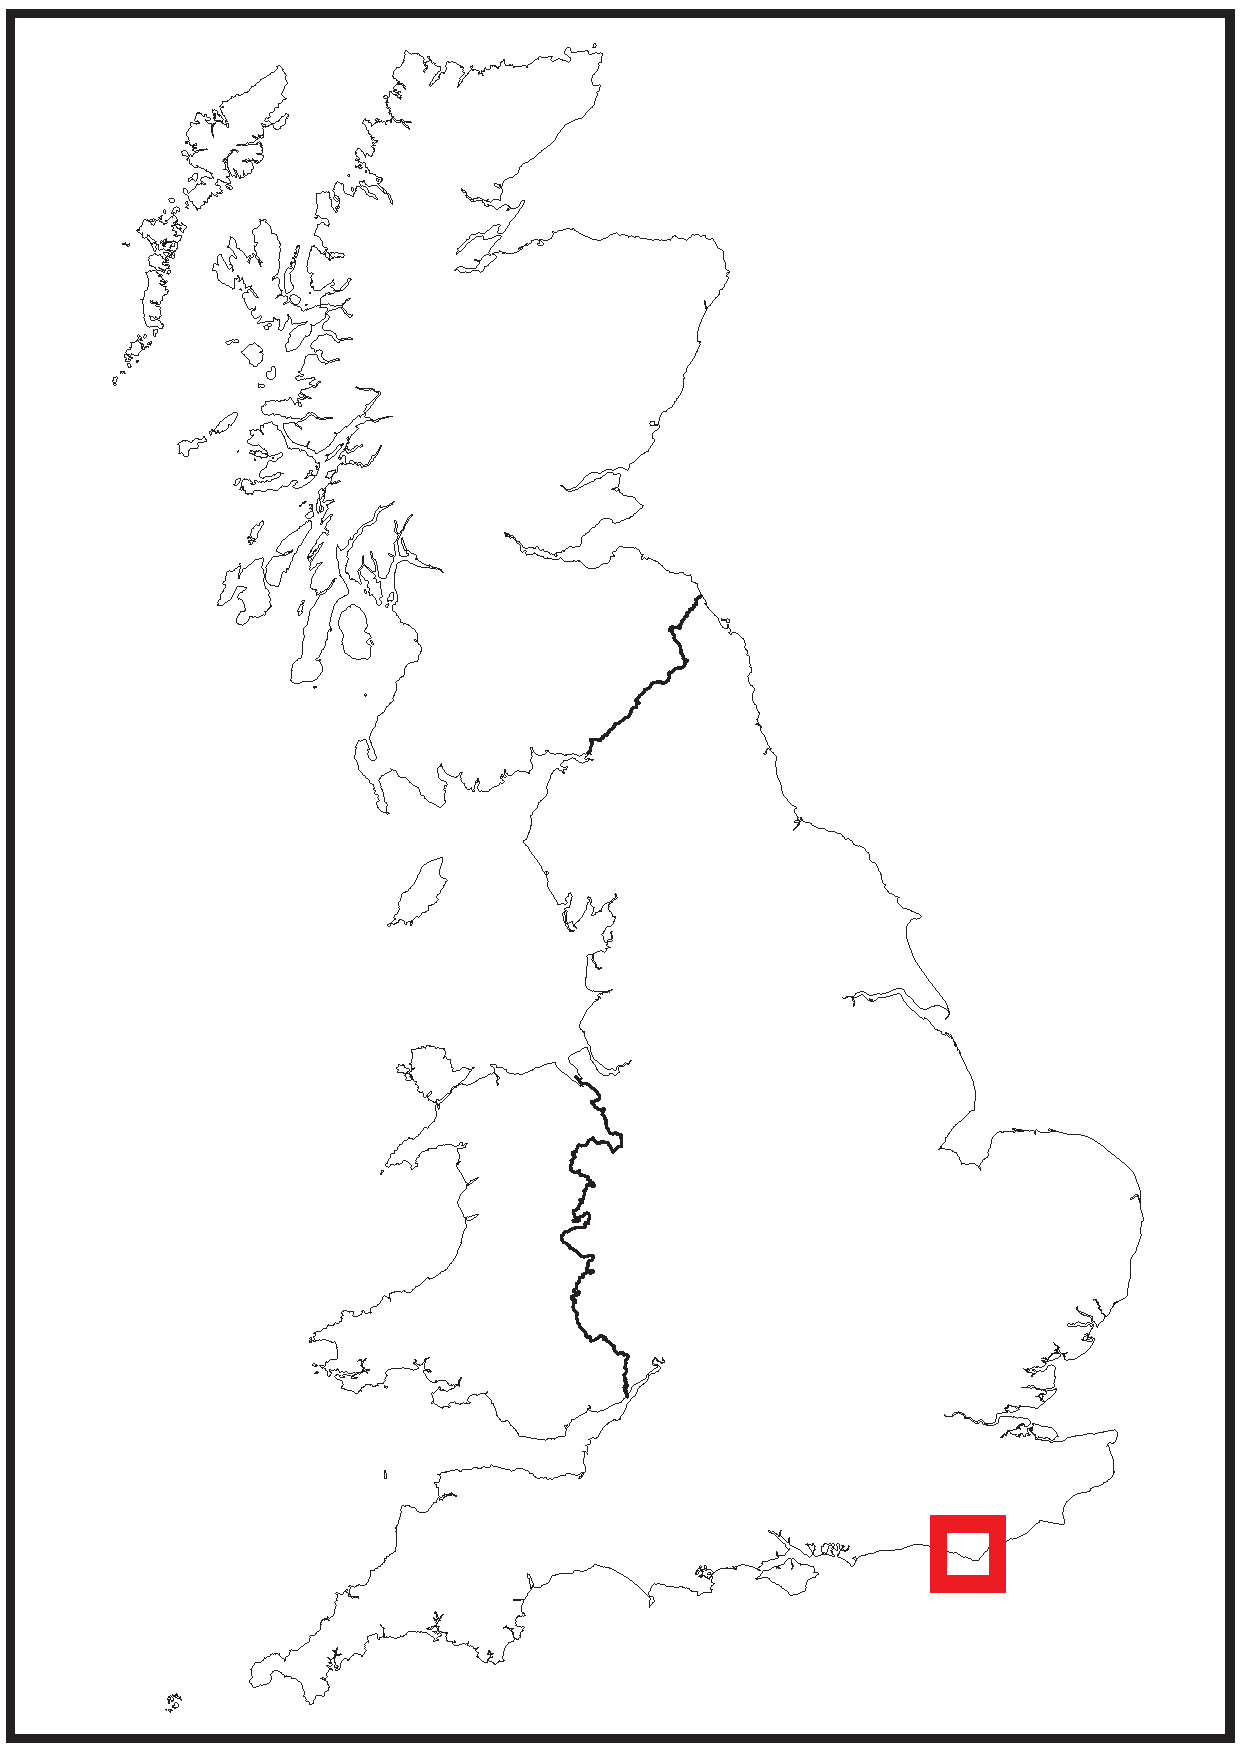
\includegraphics[width=0.19\textwidth]{./img/ukoutline}
  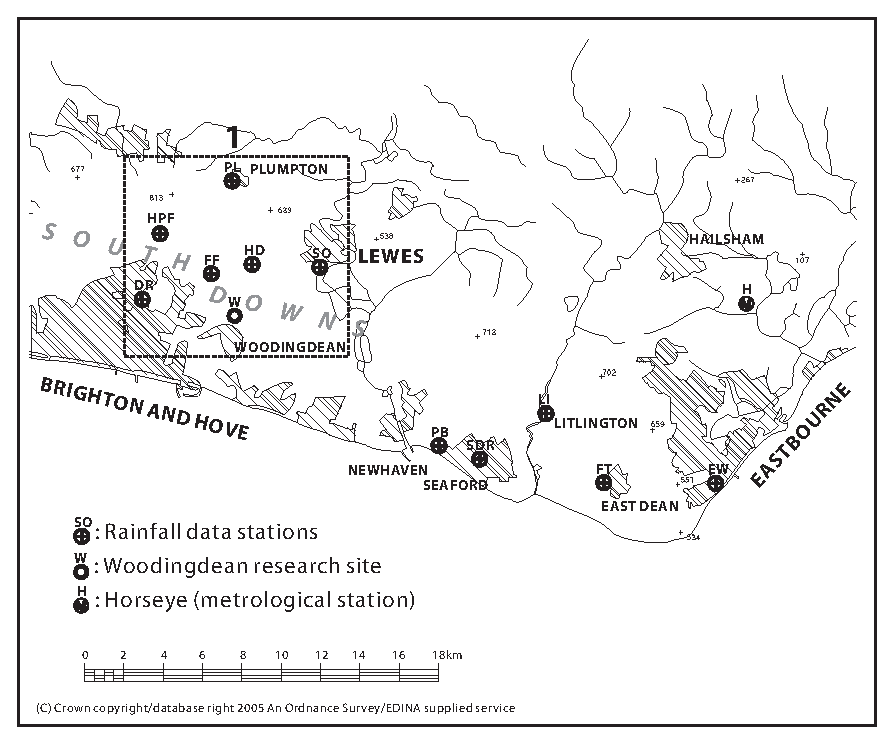
\includegraphics[width=0.8\textwidth]{./img/dailydatasite}
  \caption[Locations of daily rainfall data stations]{Locations of daily
rainfall data stations. DR: Ditchling Road, SO: Southover, PL: Plumpton, SDR:
Seaford D. Road, EW: Eastbourne Wilm., FT: Friston Tower, LI: Litlington, PB:
Poverty Bottom, HPF: High Park Farm, HD: Housedean, FF: Falmer Farm, W:
Woodingdean (soil, slope, crop management), H: Horseye (temperature);
\emph{dotted frame(1)} indicates the area shown in Figure
\ref{fig:EventRainfallDataSite}.}
  \label{fig:DailyRainfallDataSite}
\end{figure}

High resolution event rainfall data measured by tipping-bucket gauges were
obtained from three stations---Ditchling Road, Southover and Plumpton---nearby
the research site (Figure \ref{fig:EventRainfallDataSite}). Detection limit of
the tipping bucket was 0.2 mm. Data duration from each station ranged from 2 to
13 years with some missing data between 1995 and 1998. This might have been
because of vandalisms in the area, a defunct station or temporary gauge
malfunctions (personal communications with Environment Agency on 1 March 2003).
It should be noted that there are only a few rainfall stations which record
event rainfall in the study region (Figure \ref{fig:EventRainfallDataSite}).
Long term high resolution rainfall data with good quality is seldom available
because of, for example, a large size of data file. However, quality of the data
used here was reasonably good of capturing rainfall intensity details.

\begin{figure}[phtb]
  \centering
  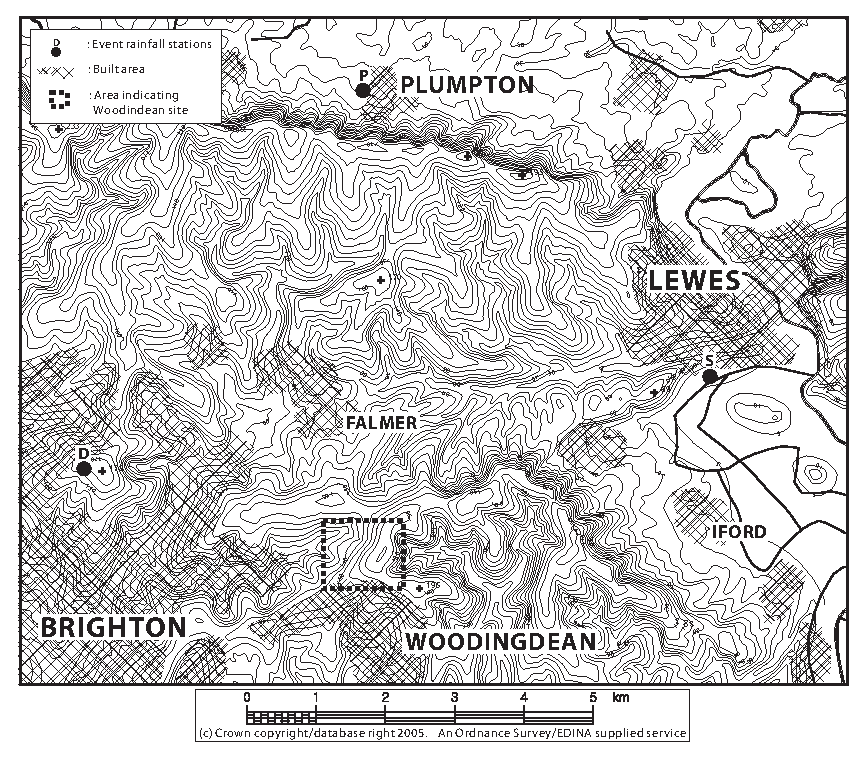
\includegraphics[width=0.8\textwidth]{./img/eventdatasite}
  \caption[Locations of event rainfall data stations]{Locations of event
rainfall data stations. \emph{filled circles}: event rainfall data stations (S:
Southover, D: Ditchling Road, P: Plumpton); Woodingdean site is indicated by
\emph{dotted frame} (see Figure \ref{fig:WoodingdeanSite} for the detail)}
  \label{fig:EventRainfallDataSite}
\end{figure}

The detailed information about the daily and event data are summarised in Table
\ref{tab:DetailsOfDataStations}.

\begin{table}[htbp]
  \figureversion{tabular}
  \centering
  \caption{Details of rainfall data stations}
  \label{tab:DetailsOfDataStations}
    \small
    \begin{tabular}{lllll}
      \toprule
      \textbf{Code} & \textbf{Station} & \textbf{Data type} &
\textbf{Grid reference} & \textbf{Periods}\\
      \midrule
      DR & Ditchling Road & daily & TQ314076 & 1980--1989\\
      SO & Southover & daily & TQ407093 & 1980--1998\\
      PL & Plumpton & daily & TQ356136 & 1980--2000\\
      SDR & Seaford D. Road & daily & TV491993 & 1980--2000\\
      EW & Eastbourne Wilm. & daily & TV611980 & 1980--2000\\
      FT & Friston Tower & daily & TV551982 & 1980--2000\\
      LI & Litlington & daily & TQ523020 & 1980--2000\\
      PB & Poverty Bottom & daily & TQ467002 & 1980--2000\\
      HPF & High Park Farm & daily & TQ331115 & 1974--2004\\
      HD & Housedean & daily & TQ369093 & 1967--2004\\
      FF & Falmer Farm & daily & TQ342084 & 1904--2002\\
      S & Southover & event & TQ407093 &
1993--2001$^\dagger$\\
      D & Ditchling Road & event & TQ315077 &
1991--2003$^\ddagger$\\
      P & Plumpton & event & TQ357135 & 2000--2002\\
      \bottomrule
%     \addlinespace[1mm]
      \multicolumn{5}{l}{\footnotesize $^\dagger$  with
missing data between Sep. 1996 to Jun. 1998}\\
      \multicolumn{5}{l}{\footnotesize $^\ddagger$  with
missing data between Feb. 1995 to Sep. 1997}
    \end{tabular}
\end{table}

\subsection{Other Data}
\label{sec:OtherData}

\subsubsection{Soil}
\label{sec:Soil}

Other input data, such as soil properties and slope profiles, were either
directly acquired from previous studies \citep{favis-mortlock1998-141} or
calibrated as shown in Table \ref{tab:HydrologicalAndErosionalParameters}.
Unless it was critically necessary, all the data were kept unchanged. This
minimizes unknown effects which may occur because of changing other erosional
factors, and also permits the present research to concentrate on the effect of
rainfall intensity changes.

The erosion simulation site is 7.7 ha in size, and is located at Drove Road,
Woodingdean (NGR: TQ358069): this is in the UK South Downs, about 6 km southwest
of Lewes (Figure \ref{fig:WoodingdeanSite}). Soil, slope and crop management
details are obtained from this site.

\begin{figure}[phtb]
  \centering
    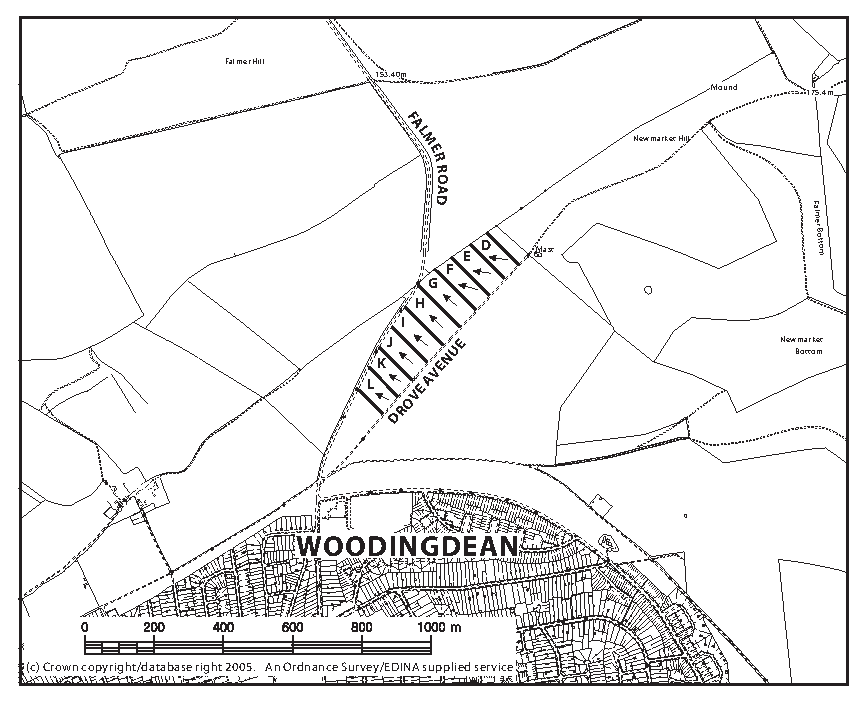
\includegraphics[width=0.8\textwidth]{./img/woodingdean}
  \caption[Woodingdean site]{Woodingdean site. The arrows indicate
approximate downslope direction. Each letter (D-L) denotes hillslope profiles
used for model simulations.}
  \label{fig:WoodingdeanSite}
\end{figure}

The soil in the area is shallow (around 20 cm to chalk) and stony silty rendzina
of the Andover series \citep{jarvis1984-soils}. The Andover silt loams of the
South Downs are both stony and prone to crusting. All the soil input parameters
are summarised in Table \ref{tab:AndoverSoilDetails} and Table
\ref{tab:HydrologicalAndErosionalParameters}.

\begin{table}[htbp]
  \figureversion{tabular}
  \centering
  \caption[Andover soil details]{Andover soil details
\citep[From][]{favis-mortlock1998-141}}
  \label{tab:AndoverSoilDetails}
    \small
    \begin{tabular}{lrrrr}\toprule
    & \multicolumn{4}{c}{Layer}\\
    \cmidrule{2-5}
    & \multicolumn{1}{c}{1} & \multicolumn{1}{c}{2} &
\multicolumn{1}{c}{3} & \multicolumn{1}{c}{4}\\
    \midrule
    Depth to bottom of layer (mm) & 150.0 & 200.0 & 300.0 & 1000.0\\
    Sand (\%) & 18.9 & 18.9 & 25.0 & 25.0\\
    Clay (\%) & 3.5 & 3.5 & 24.0 & 24.0\\
    Organic matter (\%) & 7.0 & 4.8 & 2.2 & 1.2\\
    Cation exchange capacity (meq/100 g of soil) & 45.0 & 39.0 &
30.0 & 14.0\\
    Coarse (Rock) fragments (\% vol) & 38.1 & 50.0 & 90.0 & 90.0\\
    \bottomrule
    \end{tabular}
\end{table}

Values for WEPP's parameters for effective hydraulic conductivity, together with
values for its three erodibility parameters, were subjectively adjusted
following the suggestions by \citet{favis-mortlock1998-141} (Table
\ref{tab:HydrologicalAndErosionalParameters}). The parameters for interrill and
rill erodibility ($K_i$ and $K_r$) were reduced, while the critical shear stress
parameter $\tau_c$ was increased. The value for the base line effective
hydraulic conductivity parameter $K_b$ was also increased. All the adjustments
were taken from \citet{favis-mortlock1998-141} with the exception of critical
shear stress parameter $\tau_c$ which was recalibrated to 6. This was done in
order to meet the recommended value of maximum  $\tau_c$ by the WEPP
documentation. All calibrated values were constrained to remain within the
recommended ranges in WEPP documentation \citep{flanagan1995-usda}.

\begin{table}[htbp]
  \figureversion{tabular}
  \centering
  \caption[Hydrological and erosional parameter values]{Hydrological and
erosional parameter values \citep[After][]{favis-mortlock1998-141}}
  \label{tab:HydrologicalAndErosionalParameters}
    \small
    \begin{tabular}{lrr}
    \toprule
    & Uncalibrated Hydrological & Calibrated Hydrological\\
    & and erosional parameters & and erosional parameters\\
    \midrule
    Effective hydraulic conductivity & &\\
    of top soil layer (mm/hr) & 2.1$^a$ & 3.0$^a$\\
    Interrill erodibility $K_i$ (kg s/m$^4$) & 5502700 & 2000000\\
    Rill erodibility $K_r$ (s/m) & 0.0871 & 0.0050\\
    Critical shear stress $\tau_c$ (N/m$^2$) & 3.5 & 6.0$^b$\\
    \bottomrule
%   \addlinespace[1mm]
    \multicolumn{3}{l}{\footnotesize $^a$ `baseline' effective
hydraulic conductivity for WEPP ($K_b$)}\\
    \multicolumn{3}{l}{\footnotesize $^b$ adjusted to 6 which is a
maximum value for cropland $\tau_c$}
    \end{tabular}
\end{table}

\subsubsection{Management}
\label{sec:Management}
A typical crop management practice for the area is continuous growing of winter
wheat. The typical timing of tillage operation for the area is shown in Table
\ref{tab:TillageOperationTiming}.

\begin{table}[htbp]
  \figureversion{tabular}
  \centering
  \caption[Tillage operation timing at Woodingdean site]{Tillage operation
timing at Woodingdean site \citep[From][]{favis-mortlock1998-141}}
  \label{tab:TillageOperationTiming}
    \small
    \begin{tabular}{lr@{ }l}
      \toprule
      \textbf{Operation} & \multicolumn{2}{l}{\textbf{Date}}\\
      \midrule
      Chisel plough & 20 & August\\
      Harrow & 15 & September\\
      Drill (Winter wheat) & 28 & September\\
      Roll & 1 & October\\
      Harvest & 29 & July\\
      \bottomrule
    \end{tabular}
\end{table}

\subsubsection{Topography}
\label{sec:TopographyData}
Slope angles in the site range from 12 to 20\%, with a convexity toward the
centre. The site was divided into nine sub-areas for modelling, approximately
down the line of greatest slope, which faces a northwesterly direction (Figure
\ref{fig:WoodingdeanSite}). The length of each slope varies from 125 to 180
metres, and width is 50 metres for all the slopes.

\subsubsection{Temperature}
\label{sec:Temperature}

Daily temperature records for 1990--2000 were obtained from Horseye Station
(NGR: TQ627083) (Figure \ref{fig:DailyRainfallDataSite}). The distance of this
station from the study site is about 25 km. This data set was used in this study
since no other data set was available from the region at that time. Average
annual maximum and minimum temperature are 14.9\textcelsius\ (SD:
5.5\textcelsius)\ and 6.6\textcelsius\ (SD: 4.9\textcelsius), respectively.

\section{Justification for Erosion Model Selection}
\label{sec:ModelConfiguration}

As the research aims to investigate impacts of extreme rainfall events, all soil
erosion models used in this research should be able to simulate a single erosion
event. WEPP, EUROSEM and RillGrow were chosen because of this reason. All three
models are capable of simulating single events while WEPP may also be used for
continuous simulations (Table \ref{tab:ModelsUsedInThePresentStudy}).

There are two more reasons why these models were used. One is that they use
different approaches to erosion simulations and rainfall intensity. WEPP, for
example, estimates soil erosion using steady-state approach
(Equation \ref{eq:weppsedimentload}) while EUROSEM employs a dynamic approach
using a mass balance equation (Equation \ref{eq:eurosemmassbalance}).
Both models also consider rill and interrill areas separately and use
different equations for describing processes in two areas. In terms of
rainfall intensity, WEPP uses rainfall intensity as effective rainfall
intensity for estimating interrill erosion. In EUROSEM rainfall intensity is
considered as a function of kinetic energy of raindrops which act as detachment
agents of soil particles.
RillGrow, on the other hand, is based on a
self-organising dynamic system to simulate the initiation and development of a
network of rills. RillGrow also does not consider rill and interrill areas
separately. All three models are described previously (Section
\ref{sec:SoilErosionPredictionModels}).
The other reason why these models were used is that they are
originally designed for different simulation scales, temporally and spatially.
Table \ref{tab:ModelsUsedInThePresentStudy} summarises some features of these
three models.

Comparing the outputs from three erosion models could reveal strengths and
weaknesses of their approaches to soil erosion. In turn, this investigation may
provide improved insights on the behaviour of the models in relation to rainfall
intensity changes.

\begin{sidewaystable}[htbp]
  \centering
  \caption{Summary of the erosion models used in this research}
  \label{tab:ModelsUsedInThePresentStudy}
    \begin{tabular}{llll}
\toprule
    & WEPP      & EUROSEM   & RillGrow\\
\midrule
Spatial Scale & small catchment,  & small catchment,  & small field,\\
    & hillslope,    & hillslope,  & laboratory plot\\
    & individual field  & individual field  & \\
\midrule
      Reference & \citealp{nearing1989-1587} &
\citealp{morgan1998-389} & \citealp{favis1998-353}\\
                & \citealp{flanagan1995-usda} & & \\
      \midrule
      Purpose  & event-based erosion & event-based erosion &
rill initiation\\
               & transport and deposition & transport and
deposition & and development\\
               & long-term simulation & & \\
      \midrule
      Approach & Steady-state & Dynamic & Self-organising dynamic\\
      \midrule
      Required Data & soil erodibility, & soil erodibility, &
detailed surface micro-\\
                    & slope profile & surface characteristics
& topography, soil type \\
                    & and crop management   & and plant cover
& and rainfall intensity  \\
      \midrule
      Rainfall Intensity & Yes (effective) & Yes (kinetic energy) & Yes \\
      \midrule
      Simulation Type & single event or continuous & single
event & single event\\
      \bottomrule
    \end{tabular}
\end{sidewaystable}

WEPP was selected partly because it has been widely used and studied
\citep{zhang1996-855,baffaut1998-756,favis1999-329,pruski2002-climate,
pruski2002-7,flanagan2007-1603}, so there is a substantial amount of
information to compare it with. Moreover, when WEPP was developed, it was
implemented with an unique method (or sub-model) of describing and utilizing
rainfall data, called CLIGEN. This feature has been described previously in
Section \ref{sec:ClimateGeneratorCLIGEN}. The second model, EUROSEM, was
selected because it was developed with European conditions in mind, as its name
may imply (i.e.\ \emph{EUR}opean \emph{S}oil \emph{E}rosion \emph{M}odel) (See
Section \ref{sec:EuropeanSoilErosionModelEUROSEM} for review). In this regard,
EUROSEM may provide a good comparison to WEPP, which has been developed mainly
with datasets collected from the USA \citep{flanagan2007-1603}. Lastly, RillGrow
was employed in the later stage of the research in order to generate stronger
consensus from an additional model. RillGrow's unique approach (i.e.\ a
self-organising dynamic systems approach) to soil erosion simulation (See
Section \ref{sec:ModelDescriptionRillGrow}) is also another reason for the
selection. RillGrow simulates erosion on a finer scale using iterations of
erosion estimations by a single raindrop at a time. This also gives a good
comparison to the former two models.


%
%
%$\filledstar\filledstar\filledstar$ Rationalising reason for selecting
%three models
%
%$\filledstar\filledstar\filledstar$ Contrast the models (in relation to the
%inputs as a table)
%
%\subsection{WEPP}
%\label{sec:WEPP}
%version and input data (+initial condition)
%WEPP simulation settings and assumptions.
%
%\paragraph{CLIGEN}
%\label{sec:CLIGEN}
%version and input data
%
%\begin{table}[htbp]
% \centering
% \caption[Original and Updated MEAN~P for Ditchling Road]{Original and
%Updated MEAN~P for Ditchling Road (inches)}
% \label{tab:UpdatedMEANPForDitchlingRoad}
%   \footnotesize
%   \begin{tabular}{lrrrrrrrrrrrr}
%   \toprule
%    & Jan & Feb & Mar & Apr & May & Jun & Jul & Aug & Sep & Oct &
%Nov &
%Dec\\
%   \cmidrule{2-13}
%   Original & 0.19 & 0.16 & 0.17 & 0.16 & 0.16 & 0.20 & 0.19 & 0.22
%& 0.23
%& 0.27 & 0.21 & 0.20\\
%   Updated & 0.11 & 0.11 & 0.18 & 0.21 & 0.17 & 0.15 & 0.16 & 0.13
%& 0.24 &
%0.29 & 0.19 & 0.29\\
%   \bottomrule
%   \end{tabular}
%\end{table}
%
%\begin{figure}[htbp]
% \centering
%   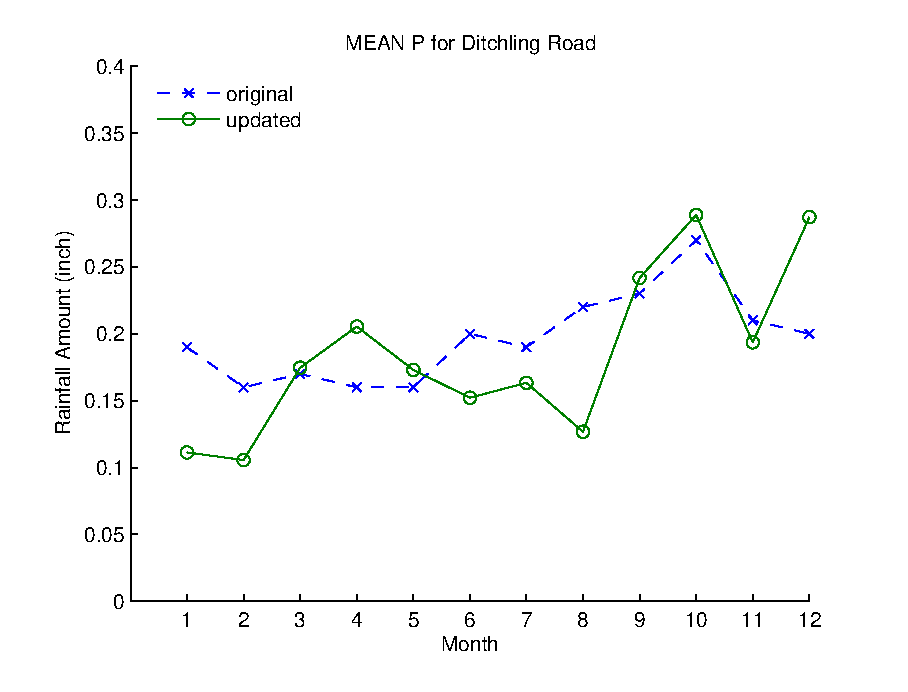
\includegraphics[width=0.60\textwidth]{mean_p_cligen}
% \caption[Mean daily precipitation depth]{Mean daily precipitation depth
%(inch)}
% \label{fig:mean_p_cligen}
%\end{figure}
%
%peak amount in autumn
%
%\begin{table}[htbp]
% \centering
% \caption[Original and Updated MX~.5P for Ditchling Road]{Original and
%Updated MX~.5P for Ditchling Road (in/hr)}
% \label{tab:UpdatedMX5PForDitchlingRoad}
%   \footnotesize
%   \begin{tabular}{lrrrrrrrrrrrr}
%   \toprule
%    & Jan & Feb & Mar & Apr & May & Jun & Jul & Aug & Sep & Oct &
%Nov & Dec\\
%   \cmidrule{2-13}
%   Original & 0.63 & 0.59 & 0.55 & 0.55 & 0.55 & 0.55 & 0.55 & 0.67
%& 0.79 & 0.93 & 0.87 & 0.75\\
%   Updated & 0.27 & 0.18 & 0.23 & 0.23 & 0.27 & 0.33 & 0.42 & 0.58
%& 0.43 & 0.45 & 0.34 & 0.30\\
%   \bottomrule
%   \end{tabular}
%\end{table}
%
%\begin{figure}[htbp]
% \centering
%   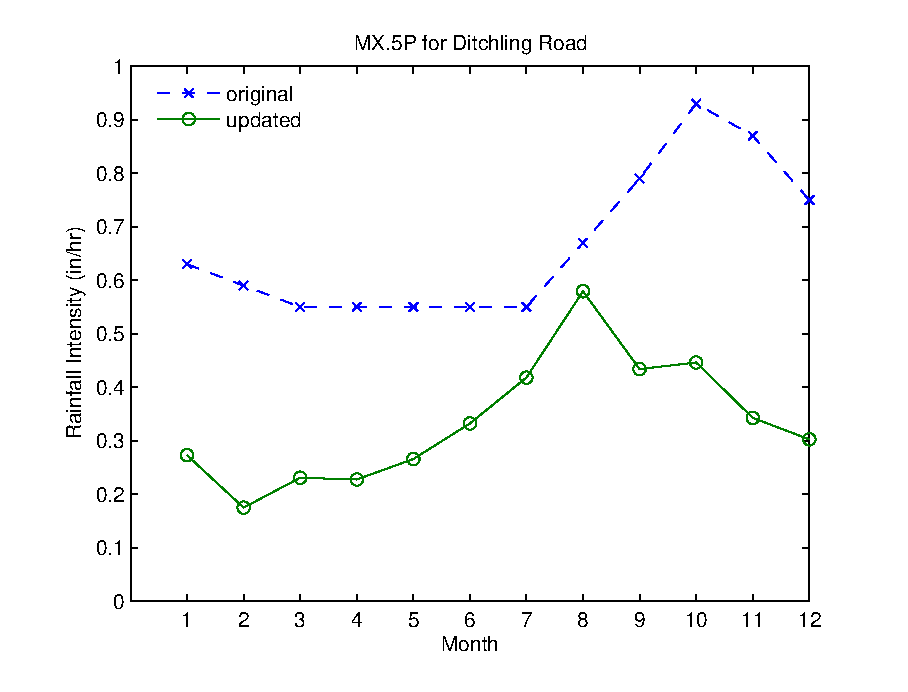
\includegraphics[width=0.70\textwidth]{mx5p_cligen}
% \caption[Mean max. daily 30-minute rainfall intensity]{Mean max. daily
%30-minute rainfall intensity (in/hr). High intensity event in summer}
% \label{fig:mx5p_cligen}
%\end{figure}
%Complete input files for both sites are shown in Appendix
%\ref{sec:CLIGENInputData}.
%
%\subsection{EUROSEM}
%\label{sec:EUROSEM}
%
%EUROSEM input settings and assumptions.
%
%\subsection{RillGrow}
%\label{sec:ModelConfigurationRillGrow}
%
%RillGrow input settings and assumptions.

\section{A Brief Overview of Research Method}
\label{sec:OverviewOfResearchMethods}

This research aims to discover how rainfall intensity changes will affect the
soil erosion rate in the future, using soil erosion models. The research method
involves data acquisition, such as observed rainfall properties and soil
properties, configuring erosion models, and sensitivity tests of erosion models.
The simulation carried out for the sensitivity test mainly employs a univariate
method.

% As this study mainly aims to investigate soil erosion changes as a response
%to future rainfall intensity changes, and future rainfall intensity changes are
%still poorly known, it is not the main focus of this study to actually attempt
%to predict future soil erosion rates. Instead, this study aims to investigate
%the way in which rainfall intensity changes can affect soil erosion rates.
%Greater knowledge here will, once future changes in rainfall intensity become
%better known, improve our ability to estimate future rates of erosion. Thus, in
%general, a ``sensitivity analysis'' approach is followed. ``Known'' rather than
%``realistic'' changes in intensity are used in this thesis.

%The thesis consists of 11 chapters in total. These chapters are divided into
%five parts: Introduction, Observed Precipitation of the Research Site, Rainfall
%Intensity Changes and Soil Erosion, Implications of Climate Change on Future
%Soil Erosion, and Conclusion.
Three soil erosion models, WEPP (Water Erosion Prediction Project), EUROSEM
(EURopean Soil Erosion Model), and RillGrow were used to simulate runoff and
erosion rate under various rainfall intensity conditions. Effects of temporal
resolution of rainfall data on runoff and soil loss generations are investigated
to identify requirements of rainfall intensity information for erosion
simulations. Two extreme rainfall events; one with highest rainfall intensity
and the other with highest rainfall amount, were selected from the
tipping-bucket rainfall data. Tipping-bucket data for the events are then
aggregated into a range of different temporal ``scales". This is done by the
discretization of tipping-bucket data into rainfall data that have a range of
time-steps (i.e. 1, 5, 15, 30 and 60min).
Runoff and soil loss rates were simulated using three models with these rainfall
input data. An additional rainfall event, which has both wet and dry phases
during the storm period, was selected. Two rainfall input data were prepared
from this event data; one without any alteration and the other that is
aggregated into a continuous storm by removing dry phases during the storm.
Runoff and soil loss rates were simulated using three models with these two
additional rainfall inputs. This was done to investigate effects of the dry
phase within a storm on soil erosion. Impacts of various rainfall intensities
patterns on soil erosion were also studied using rainfall data from a designed
storm. Four different storms that have increasing, increasing-decreasing,
decreasing and constant rainfall intensity were prepared for erosion
simulations. Rainfall amounts for all four storms were kept the same while the
intensities vary.

To understand observed trends of rainfall intensity changes, three observed
precipitation data (i.e.\ Monthly 0.5\textdegree\ grid data, daily station data
and tipping-bucket gauge data) were acquired from the South Downs, UK. Monthly
0.5\textdegree\ grid data for 100 years were analysed, firstly, to draw outlines
of long term rainfall trends in the area. Daily precipitation data from 11
stations for the various observational periods (i.e.\ 9--93 years) in the area
were then analysed, in terms of:
\begin{itemize*}
 \item daily rainfall amount,
 \item number of raindays,
 \item simple daily intensity index,
 \item number of raindays with rainfall amount $\geq$10 mm, and
 \item number of raindays with rainfall amount $\geq$20 mm.
\end{itemize*}
This gave more detailed information about the trends of rainfall in the region
than that obtained from monthly 0.5\textdegree\ grid data. Lastly, even greater
detailed rainfall trends were studied using tipping-bucket collected rainfall
data from three stations over the period of 2--13 years. This kind of high
resolution data provides very detailed information on the patterns of the
rainfall amount and intensity.

Likely future soil erosion rates were estimated only using WEPP, as the other
two models are not designed for continuous long term simulations. A hundred
year-long weather is generated by the WEPP's climate component called CLIGEN
(CLImate GENerator) as a control climate dataset. Rainfall intensity was
then increased proportionally from the control data by changing rainfall
duration, keeping rainfall amount constant. Runoff and erosion rates were
simulated using these climate data.

\subsection{Statistical Methods for Trend Investigation}
\label{StatisticalMethodsForTrendInvestigation}

Statistical methods used in this research are briefly summarized here.

\paragraph{Simple Linear Regression}
\label{sec:SimpleLinearRegression}

%REGRESSION OR CORRELATION?
%
%Select the Pearson (parametric) correlation coefficient if you can assume
%that both X and Y are sampled from Gaussian populations. Otherwise choose
%the Spearman nonparametric correlation coefficient. Don't calculate the
%correlation coefficient (or its confidence interval) if you manipulated the
%X variable.

%Calculate linear regressions only if one of the variables (X) is likely to
%precede or cause the other variable (Y). Definitely choose linear
%regression if you manipulated the X variable. It makes a big difference
%which variable is called X and which is called Y, as linear regression
%calculations are not symmetrical with respect to X and Y. If you swap the
%two variables, you will obtain a different regression line.

Linear regression function ($y=\alpha + \beta x$) was assumed where rainfall
related indicators (Table \ref{tab:RainfallIntensityIndicators}) as dependent
variables ($y$) and time as a independent variable ($x$). The regression
coefficient ($\beta$) might be used to detect trends in time series of the
indicators. The Student's $t$-test was used to test whether the trend is
statistically significant.

%If $t$-value is greater than 1.96 ($n=\infty$), reject null hypothesis
%($\beta = 0$) with $95\%$ confidence level.
%If $n=5$, $\bar{x}\pm2.776 \frac{\sigma}{n^{1/2}}$ ; if N=10: Xavg$\pm$
%2.262 sdev/N1/2 ; if N=20: Xavg$\pm$ 2.093 sdev/N1/2 ; if N=40; Xavg$\pm$
%2.023 sdev/N1/2 ; and for ``arge'' N: Xavg$\pm$ 1.960 sdev/N1/2


\paragraph{Mann-Kendall's Test}
\label{sec:MannKendallSTest}

Mann-Kendall's test is a non-parametric test for the detection of trend in a
time series. This is primarily used because it has no linearity assumption.
Since the first proposals of the test by \citet{mann1945-245} and
\citet{kendall1975-202}, covariances between Mann-Kendall statistics were
proposed by \citet{dietz1981-169} and the test was extended in order to include
seasonality \citep{hirsch1984-727}, multiple monitoring sites
\citep{lettenmaier1988-505} and covariates representing natural fluctuations
\citep{libiseller2002-71}.

%This section should be about Kendall's rank correlation.
%look at the matlab script!

The Mann-Kendall rank correlation \citep{mann1945-245,kendall1975-202} is
sensitive to both linear and non-linear trends. This is a non-parametric method
and is based on ranking of a time series, using only the relative ordering of
ranks \citep{press1996-933}. It does not give any information about the
magnitude of the trend in the actual time series but rather gives a significance
of the trend, and information on the direction of the observed trend (i.e.\
upward, downward or unchanged).

%\begin{equation}
%\label{eq:Tau}
% T=\sum^{N}_{i=1}n_i
%\end{equation}
%where, $N$ is the total number of element in the data set (no. of years).
%$n_i$ is the number of preceding element that is larger than element $x_i$
%(i=1,2,\ldots $N$).
%When $N$ is greater than 10, the distribution function of $T$ (test
%variable) is assumed to be asymptotically Gaussian.
%
%Thus, expected value, $E(T)$ is given by:
%
%\begin{equation}
%\label{eq:ExpectedTau}
% E(T)=\mu=\frac{N(N-1)}{4}
%\end{equation}
%and, variance, $var(T)$ is given by:
%
%\begin{equation}
%\label{eq:VarianceTau}
% var(T)=\sigma^2=\frac{N(N-1)(2N+5)}{72}
%\end{equation}
%The normalised test variable, $Z(T)$, is given by:
%
%\begin{equation}
%\label{eq:NormalisedTestVariable}
% Z(T)=\frac{T-E(T)}{\sqrt{var(T)}}
%\end{equation}
%
%If $|Z(T)| > 1.96$, $H_0$ shall be rejected with $95\%$ confidence level.
%When $Z(T)$ is significant, $Z(T) > 0$ or $Z(T) < 0$ defines an ascending
%or descending trend.

\paragraph{Kolmogorov-Smirnov test}
\label{sec:KolmogorovSmirnovTest}
The two sample Kolmogorov-Smirnov test is used to determine if two distributions
differ significantly. The K-S test is a non-parametric test that tests
differences between two distributions. The K-S test has the advantage of making
no assumption about the distribution of data. Its null hypothesis is that the
two samples are distributed identically. The test is sensitive to differences in
location, dispersion and skewness of the distribution \citep{sokal1995-887}.

%\begin{verbatim}
%http://en.wikipedia.org/wiki/Kolmogorov-Smirnov_test
%\end{verbatim}
%09:06, 13 September 2006
%
%$\downarrow$ need to be reworded
%
%In statistics, the Kolmogorov-Smirnov test (often called the K-S test) is
%used to determine whether two underlying probability distributions differ,
%or whether an underlying probability distribution differs from a
%hypothesized distribution, in either case based on finite samples.
%
%The one-sample KS test compares the empirical distribution function with
%the cumulative distribution function specified by the null hypothesis. The
%main applications are testing goodness of fit with the normal and uniform
%distributions. For normality testing, minor improvements made by Lilliefors
%lead to the Lilliefors test. In general the Shapiro-Wilk test or
%Anderson-Darling test are more powerful alternatives to the Lilliefors test
%for testing normality.
%
%The two-sample KS test is one of the most useful and general nonparametric
%methods for comparing two samples, as it is sensitive to differences in
%both location and shape of the empirical cumulative distribution functions
%of the two samples.
%
%empirical distribution function Fn for n observations yi is defined as
%
%\begin{equation}
% F_n(x)={\frac{1}{n}}\sum_{i=1}^n \left\{\begin{matrix}1 & \mathrm{if}\
%y_i\leq x, \\ 0 & \mathrm{otherwise}.\end{matrix}\right.
%\end{equation}
%
%The two one-sided Kolmogorov-Smirnov test statistics are given by
%
%\begin{equation}
% D_n^{+}=\max(F_n(x)-F(x))
%\end{equation}
%\begin{equation}
%     D_n^{-}=\max(F(x)-F_n(x))
%\end{equation}
%
%where F(x) is the hypothesized distribution or another empirical
%distribution. The probability distributions of these two statistics, given
%that the null hypothesis of equality of distributions is true, does not
%depend on what the hypothesized distribution is, as long as it is
%continuous.
%
%Knuth gives a detailed description of how to analyse the significance of
%this pair of statistics [citation needed]. Many people use max(Dn+, Dn-)
%instead, but the distribution of this statistic is more difficult to deal
%with.
%
%
%When the underlying independent variable is cyclic, as with day of the year
%or day of the week, then Kuiper's test is more appropriate. Numerical
%Recipes is a good source of information on this.
%
%Furthermore, the Kolmogorov-Smirnov test is more sensitive at points near
%the median of the distribution than at its tails. The Anderson-Darling test
%provides equal sensitivity at the tails.

%******This part may need to be more descriptive
%
%The research described here involves three strategic stages:
%\begin{quote}
% \begin{enumerate}
%   \item Investigation of Rainfall Intensity
%   \item Erosion Model Evaluation
%   \item Estimation of Future Soil Erosion
% \end{enumerate}
%\end{quote}
%
%For the first stage, three temporally and spatially different datasets
%(i.e.\ monthly 0.5\textdegree\ grid data, daily station data and
%tipping-bucket gauge data) are investigated to find trends in rainfall
%intensity changes.
%In the second stage, Erosion Model Evaluation assesses soil erosion models
%(e.g.\ WEPP and EUROSEM) to find out their responses to rainfall intensity
%changes. The changes in rainfall intensity are accomplished by changing the
%original intensity proportionally. This stage provides information on
%differences between the models' responses compared to real erosion system's
%responses to changed rainfall intensity.
%At the final stage, the outcomes from the previous two stages provide
%information on future rainfall intensity, and erosion model response to
%rainfall intensity changes. This information is then used to estimate
%likely ranges of future rainfall intensity changes. In turn, future soil
%erosion rate are estimated.
%
%This research may expect following outcomes:
%\begin{quote}
% \begin{enumerate}
%   \item Improvement of our understandings of rainfall intensity
%   \item Requirement of rainfall intensity information for soil
%erosion estimation
%   \item Identification of limitations of soil erosion models for
%incorporating future rainfall intensity changes
%   \item Suggestions for soil erosion model improvements
%   \item Estimation of future soil losses induced by rainfall
%intensity changes
% \end{enumerate}
%\end{quote}

%\nolinenumbers
